\documentclass[11pt]{article}

\usepackage{graphicx}
\usepackage{amssymb}
\usepackage{color}
\usepackage{hyperref}
\usepackage[utf8]{inputenc}

\begin{document}

\begin{center}
\includegraphics[scale=0.25]{fit_logo.png}
$$$$
{\LARGE Semestrální projekt IEL 2016/2017 \par}
$$$$
{\Large 1. Listopadu 2016 \par}
\end{center}

$$$$$$$$$$$$$$$$$$$$$$$$$$$$$$$$$$$$$$$$$$$$

Autor: Filip Kočica,\href{mailto:xkocic01@fit.vutbr.cz}{xkocic01@fit.vutbr.cz}

\quad \quad \quad Fakulta informačních technologií

\quad \quad \quad Vysoké učení technické v Brně

\begin{center}

{\Large První úloha, Varianta F: Stanovte pomocí metody zjednodušování \color{red} U_R_8, I_R_8 \par}
\begin{center}
    \begin{tabular}{ | l | l | l | l | l | l | l | l | l | l |}
    \hline
    U1[V] & U2[V] & R1[\Omega] & R2[\Omega] &R3 [\Omega] &R4 [\Omega] & R5[\Omega] & R6[\Omega] & R7[\Omega] & R8[\Omega] \\ \hline
    125 & 65 & 510 & 500 & 550 & 250 & 300 & 800 & 330 & 250 \\ \hline
   
    \end{tabular}
\end{center}


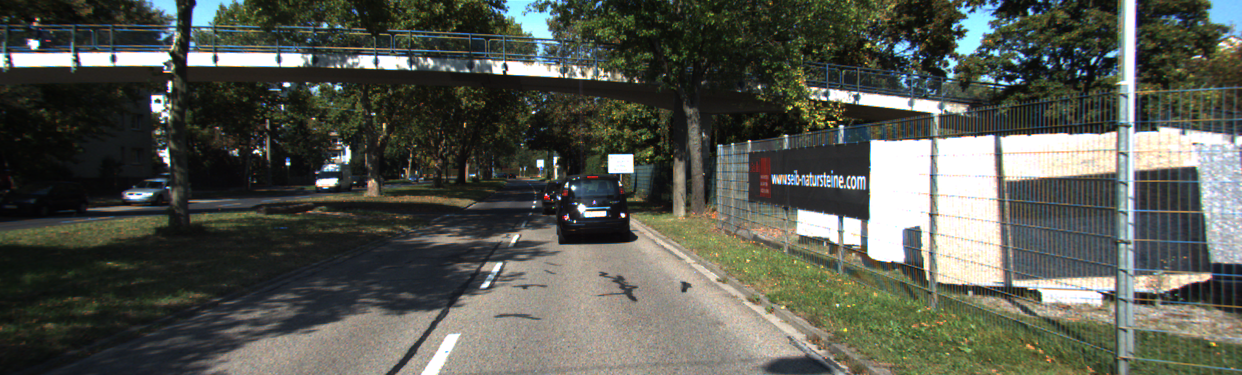
\includegraphics[scale=0.5]{1.png}
\end{center}

Výpočet dvou sériově zapojených zdrojů:

$$U = U_1 + U_2 = 125 + 65 = 190V$$

Výpočet dvou paralelně zapojených odporů:

$$R_7_8=\frac{R_7R_8}{R_7+R_8}=\frac{330*250}{330+250}=142.2414\Omega$$

Převod trojúhelník-hvězda:

$$R_A=\frac{R_1R_2}{R_1+R_2+R_3}=\frac{510*500}{510+500+550}=163.4615\Omega$$
$$R_B=\frac{R_1R_3}{R_1+R_2+R_3}=\frac{510*550}{510+500+550}=179.8077\Omega$$
$$R_C=\frac{R_2R_3}{R_1+R_2+R_3}=\frac{500*550}{510+500+550}=176.2820\Omega$$

\begin{center}
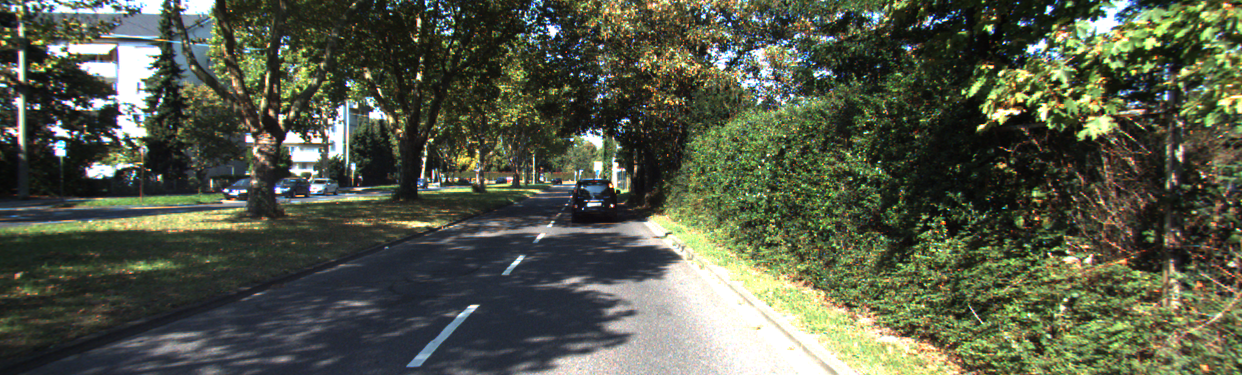
\includegraphics[scale=0.5]{2.png}
\end{center}
Součet sériově zapojených odporů:

$$R_B_4=R_B+R_4=429.8077\Omega$$
$$R_C_5=R_C+R_5=476.2820\Omega$$
$$R_6_7_8=R_6+R_7_8=942.2414\Omega$$

$$$$
\begin{center}
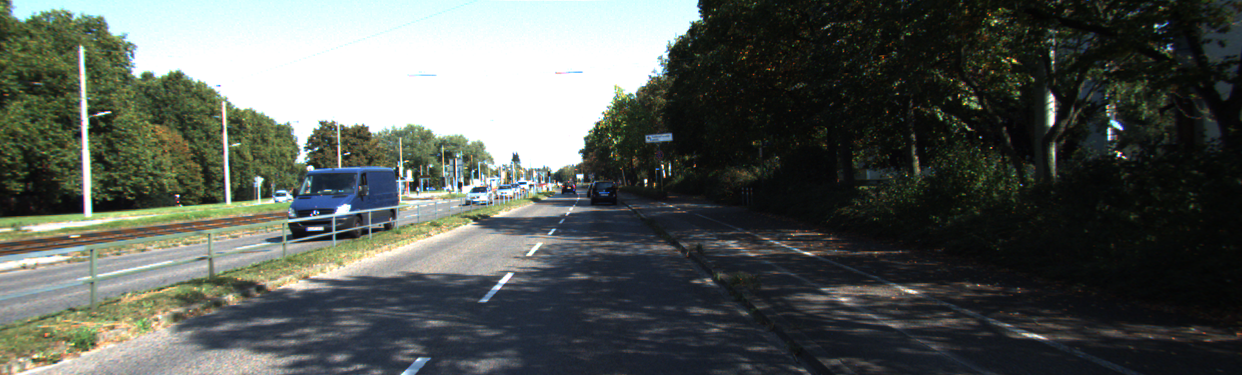
\includegraphics[scale=0.5]{3.png}
\end{center}
Součet paralelně zapojených odporů:

$$R_B_4_C_5=\frac{R_B_4R_C_5}{R_B_4+R_C_5}=\frac{429.8077*476.282}{429.8077+476.282}=225.9265\Omega$$


\begin{center}
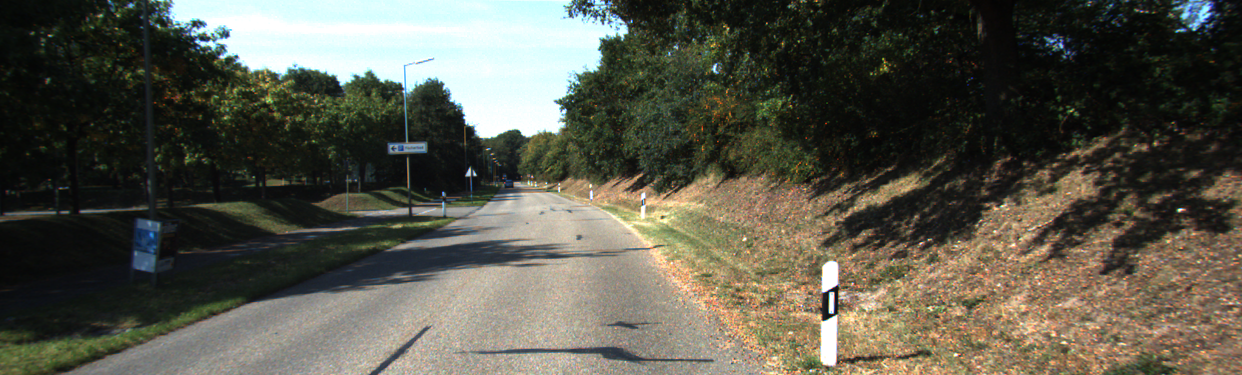
\includegraphics[scale=0.5]{4.png}
\end{center}
Součet sériově zapojených odporů:

$$R_E_K_V=R_A+R_B_4_C_5+R_6_7_8=1331.6294\Omega$$
\begin{center}
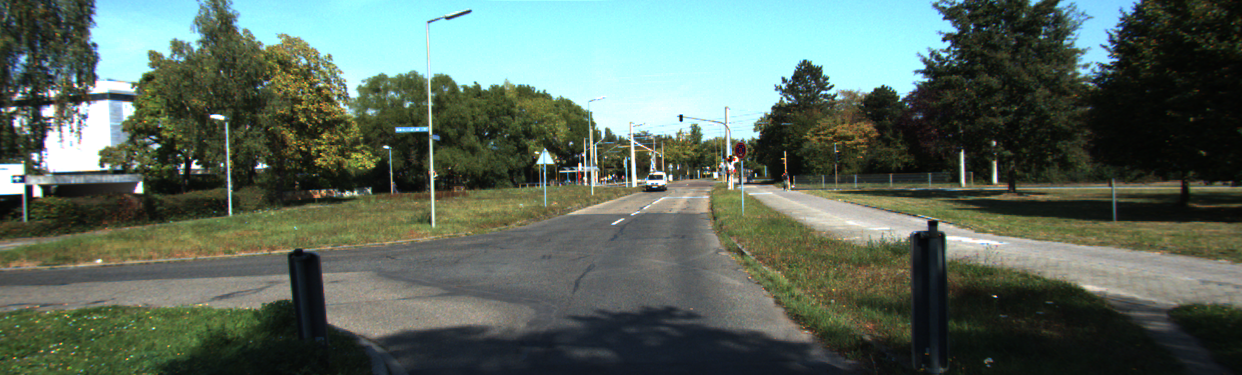
\includegraphics[scale=0.5]{5.png}
\end{center}
Výpočet proudu procházejícího obvodem:

$$I=\frac{U}{R_E_K_V}=0.1427A$$



\begin{center}
{\Large \color{red} ROZŠÍŘENÍ \par}
\end{center}

\begin{center}
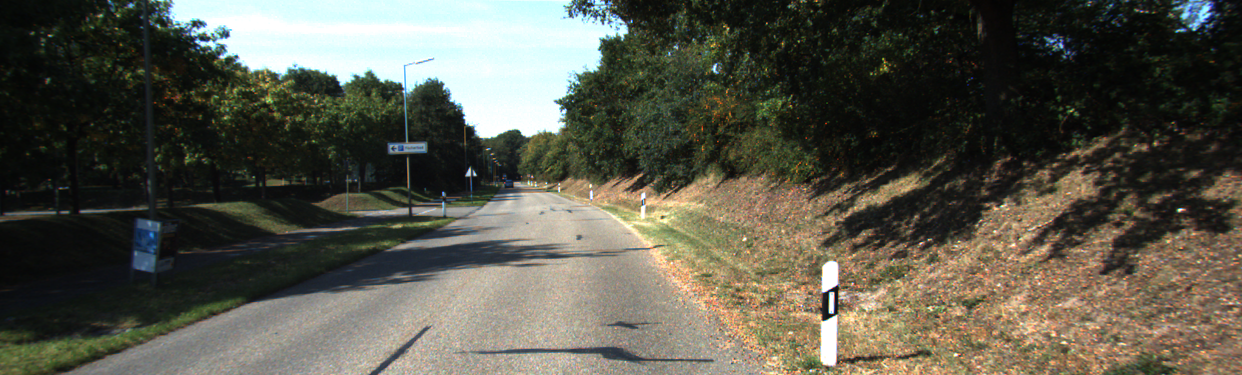
\includegraphics[scale=0.5]{4.png}
\end{center}
$$U_R_A=R_A*I=0.1427*163.4615=23.3260V$$
$$U_R_6_7_8=R_6_7_8*I=0.1427*942.2414=134.4578V$$
$$U_R_B_4_C_5=R_B_4_C_5*I=0.1427*225.9265=32.2397V$$

Kontrola pomocí II.KZ:

$$U-U_R_A-U_R_6_7_8-U_R_B_4_C_5=0$$
$$190-23.3260-134.4578-32.2397=0$$
$$190-190=0$$
$$0=0$$


$$$$
\begin{center}
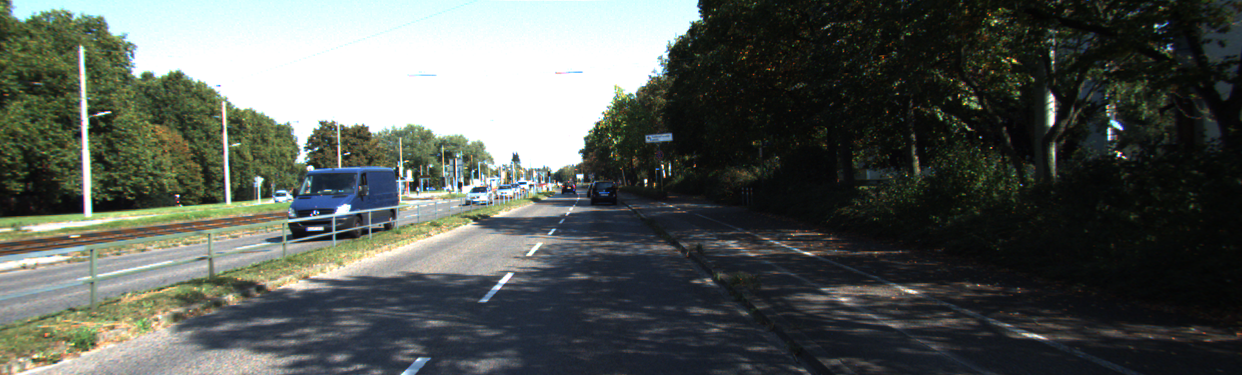
\includegraphics[scale=0.5]{3.png}
\end{center}
$$$$
Výpočet proudů, které se větví do R_B_4  -a-  R_C_5

$$I_1=\frac{U_R_B_4_C_5}{R_B_4}=\frac{32.2397}{429.8077}=0.075A$$
$$I_2=\frac{U_R_B_4_C_5}{R_C_5}=\frac{32.2397}{476.2820}=0.0677A$$$$$$

Kontrola pomocí I.KZ:

$$I-I_1-I_2=0$$
$$0.1427-0.075-0.0677=0$$
$$0=0$$


\begin{center}
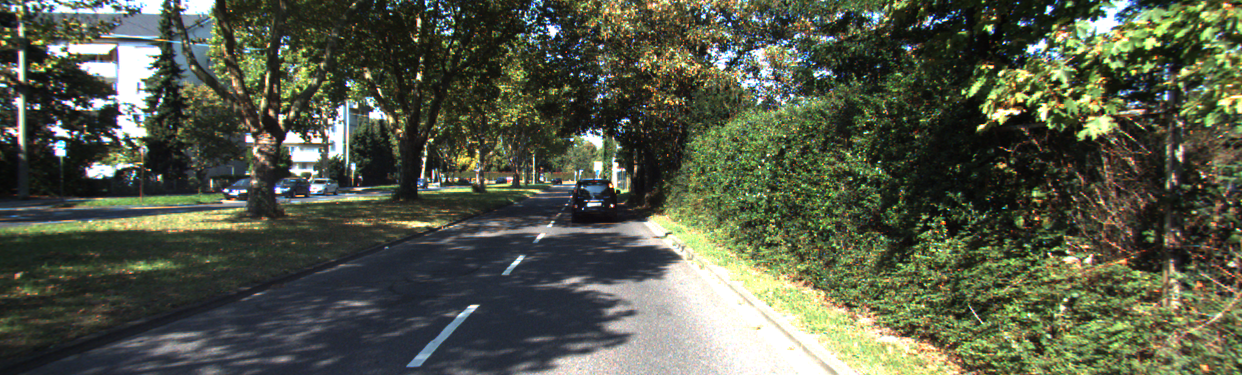
\includegraphics[scale=0.5]{2.png}
\end{center}

$$$$
Výpočty úbytků napětí na jednotlivých odporech:

$$U_R_B=I_1*R_B=0.075*179.8077=13.4856V$$
$$U_R_4=I_1*R_4=0.075*250=18.75V$$
$$U_R_C=I_2*R_C=0.0677*176.2820=11.9343V$$
$$U_R_5=I_2*R_5=0.0677*300=20.31V$$
$$U_R_6=I*R_6=0.1427*800=114.16V$$
$$U_R_7_8=I*R_7_8=0.1427*142.2414=20.2978V$$

$$$$
Kontrola pomocí II.KZ (Na paralelně zapojených odporech je vždy stejné napětí):

$$U_R_B+U_R_4-U_R_B_4_C_5=0$$
$$13.4856+18.75-32.2356=0$$
$$0=0$$
$$U_R_C+U_R_5-U_R_B_4_C_5=0$$
$$20.31+11.9343-32.2356=0$$
$$0=0$$
$$U_R_6_7_8-U_R_6-U_R_7_8=0$$
$$134.4578-114.16-20.2978=0$$
$$0=0$$

$$$$
Výpočet proudů větvících se do R_7 -a- R_8

$$I_3=\frac{U_R_7_8}{R_7}=\frac{20.2978}{330}=0.0615A$$
$$I_4=\frac{U_R_7_8}{R_8}=\frac{20.2978}{250}=0.0812A$$$$$$

Kontrola pomocí I.KZ

$$I-I_3-I_4=0$$
$$0.1427-0.0615-0.0812=0$$
$$0=0$$


Hledané I_R_8 -a- U_R_8

$$I_R_8=I_4=0.0812A$$
$$U_R_8=I_R_8 * R_8 = 250 * 0.0812 = 20.3V$

$$$$$$$$$$$$$$$$$$$$$$$$$$$$$$$$$$$$

\begin{center}

{\Large Druhá úloha, Varianta D: Stanovte pomocí Theveninova teorému \color{red} U_R_4, I_R_4 \par}

$$$$
    \begin{tabular}{ | l | l | l | l | l | l |}
    \hline
    U[V] & R1[\Omega] & R2[\Omega] &R3 [\Omega] &R4 [\Omega] & R5[\Omega] \\ \hline
    150 & 200 & 660 & 200 & 550 & 330 \\ \hline
   
    \end{tabular}

$$$$
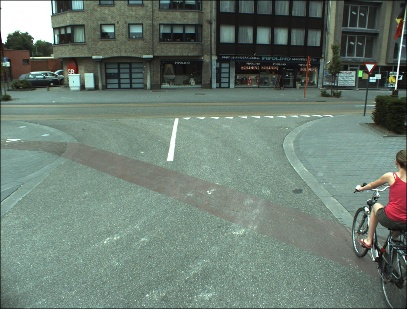
\includegraphics[scale=0.5]{6.png}
\end{center}

$$R_3_5 = R_3 + R_5 = 200 + 330 = 530\Omega$$


$$R_2_3_5 = \frac{R_2R_3_5}{R_2+R_3_5}=\frac{660*530}{660+530}=293.9496\Omega$$


$$R_1_2_3_5 = R_1 + R_2_3_5=200+293.9496=493.9496\Omega$$


$$I_1 = \frac{U}{R_1_2_3_5} = \frac{150}{493.9496} = 0.3037A$$

$$U_R_1 = R_1 * I_1 = 0.3037 * 200 = 60.74V$$

$$U_R_2 = U - U_R_1 = 150-60.74=89.26V$$

$$I_2 = \frac{U_R_2}{R_2} = \frac{89.26}{660}=0.1352A$$

$$I_3 = I_1 - I_2 = 0.3037-0.1352=0.1685A$$
\begin{center}
\includegraphics[scale=0.5]{7.png}
\end{center}

$$U_i = I_3 * R_3 = 200 * 0.1685 = 33.7V$$

$$R_i = \frac{[(\frac{R_1R_2}{R_1+R_2})+R_5] * R_3}{[(\frac{R_1R_2}{R_1+R_2})+R_5] + R_3} =\frac{(153.4884 + 330) * 200}{153.4884 + 330 + 200}=\frac{96697.68}{683.4884}=141.4767\Omega$$

$$I_R_4 = \frac{U_i}{R_i+R_4}=\frac{33.7}{141.4767+550}=0.0487A$$

$$U_R_4=R_4*I_R_4=550*0.0487=26.785V$$

$$$$$$$$

\begin{center}

$$$$$$$$$$$$$$$$
$$$$$$$$$$$$$$$$
{\Large Třetí úloha, Varianta D: Stanovte pomocí metody uzlových napětí \color{red} U_R_4, I_R_4 \par}


    \begin{tabular}{ | l | l | l | l | l | l | l | l |}
    \hline
    U[V] & I1[A] & I2[A] & R1[\Omega] & R2[\Omega] &R3 [\Omega] &R4 [\Omega] & R5[\Omega] \\ \hline
    115 & 0.6 & 0.9 & 50 & 38 & 48 & 37 & 28 \\ \hline
   
    \end{tabular}

\includegraphics[scale=0.6]{8.png}

Sestavíme rovnice pro uzly A, B, C.
$$A: I_2 - I_R_1 + I_R_2 = 0$$
$$B: I_R_5 - I_R_3 - I_R_2 = 0$$
$$C: I_R_3 - I_R_5 - I_R_4 = 0$$
Pomocí II. Kirchhofova zákona sestavíme rovnice pro proudy:
$$R_1 * I_R_1 - U_A = 0 -> I_R_1 = \frac{U_A}{R_1}$$
$$R_2 * I_R_2 + U_B - U_A = 0 -> I_R_2 = \frac{U_A - U_B}{R_2}$$
$$R_3 * I_R_3 + U_C - U_B = 0 -> I_R_3 = \frac{U_B - U_C}{R_3}$$
$$R_4 * I_R_4 - U_C = 0 -> I_R_4 = \frac{U_C}{R_4}$$
$$R_5 * I_R_5 + U_3 + U_B - U_C = 0 -> I_R_5 = \frac{U_C - U_B - U_3}{R_5} $$
$$$$

\end{center}
$$$$

\begin{center}



{\Large Čtvrtá úloha, Varianta F: Pro napájecí napětí platí: $$u_1 = U_1*sin(2\pi ft)$$
$$u_2 = U_2*sin(2\pi ft)$$
Ve vztahu pro napětí $$u_C_1 = U_C_1*sin(2πf t+ϕC1)$$
stanovte pomocí metody smyčkových proudů
 \color{red} $$|U_C_1|, \phi _C_1$$ \par}
    \begin{tabular}{ | l | l | l | l | l | l | l | l |}
    \hline
    U[V] & I1[A] & I2[A] & R1[\Omega] & R2[\Omega] &R3 [\Omega] &R4 [\Omega] & R5[\Omega] \\ \hline
    115 & 0.6 & 0.9 & 50 & 38 & 48 & 37 & 28 \\ \hline
   
    \end{tabular}
\end{center}
$$$$

$$$$$$$$$$$$$$$$$$$$$$$$$$$$$$$$$$$$$$$$$$$$$$$$$$$$

{\Large Pátá úloha, Varianta D: Sestavte diferenciální rovnici popisující chování obvodu na obrázku, dále ji
upravte dosazením hodnot parametrů. Vypočítejte analytické řešení \color{red}i_L = f(t).\par}{\Large Provedte kontrolu výpočtu dosazením do sestavené diferenciální rovnice.\par}
$$$$
\begin{center}
    \begin{tabular}{ | l | l | l | l |}
    \hline
    U[V] & L[H] & R[\Omega] & i_L (0)[A] \\ \hline
    50 & 5 & 25 & 6 \\ \hline
   
    \end{tabular}
\end{center}

$$$$$$$$
\begin{center}
\includegraphics[scale=0.6]{uloha5.png}
\end{center}

$$i_L' = \frac{1}{L}  * u_L

$$i_L * R + u_L - U = 0

$$i_L' = \frac{1}{L} * (U - R * i_L)

$$i_L' = \frac{1}{5} * (50 - 25 * i_L)

$$i_L' = 10 - 5*i_L

$$i_L' + 5*i_L = 10

I. Počáteční podmínka:

$$i_L(0) = 6

II. Očekávané řešení:

$$i_L(t) = L(t) * e^\lambda^t

III. Výpočet lambdy:

$$\lambda + 5 = 0

$$\lambda = -5

IV.Dosazení do rovnice:

$$i_L(t) = L(t) * e^-^5^t

Vyrobíme i_L':

$$i_L' = L(t)' * e^-^5^t + L(t) * e^-^5^t * (-5)

Dosadíme do rovnice:

$$L(t)' * e^-^5^t - 5 * (L(t) * e^-^5^t) + 5 * (L(t) * e^-^5^t) = 10

$$L(t)' = 10 / e^-^5^t

$$L(t)' = 10 * e^5^t / \int

$$L(t) + K_1 = 2 * e^5^t + K_2

$$L(t) = 2 * e^5^t + K

Dosadím do rovnice:

$$i_L = L(t) * e^-^5^t

$$i_L = (2 * e^5^t + K) * e^-^5^t

$$i_L = 2 * e^5^t^-^5^t + K * e^-^5^t

$$i_L = 2 + K * e^-^5^t

$$ 6 = 2 + K * e^-^5^*^0

$$ 6 - 2 = K * 1

$$K = 4

$$i_L = 2 + 4 * e^-^5^t

Zkoušky:

$$1. i_L(0) = 2 + 4 * e^-^5^*^0

$$6 = 6 => Splněno

$$2. i_L' + 5 * i_L = 10

$$i_L' = - 20 e^-^5^t

$$-20 * e^-^5^t + 5 * (2 + 4 * e^-^5^t) = 10

$$10 = 10 => Splněno


$$$$$$$$$$$$$$$$
\begin{center}
{\Large Souhrn výsledků \par}
$$$$
    \begin{tabular}{ | l | l | l |}
    \hline
    Příklad č. & Varianta & Výsledek \\ \hline
   		1 & F & I_R_8 = 0.0812A	,	U_R_8 = 20.3V \\ \hline
    	2 & D & I_R_4 = 0.0487A	,	U_R_4 = 26.785V \\ \hline
    	3 & D & I_R_4 = A,		U_R_4 = V \\ \hline
    	4 & F & | U_C_1| = ,		\phi _C_1 = \\ \hline
    	5 & D & i_L = 2 + 4 * e^-^5^t\\ \hline
    \end{tabular}
\end{center}

\end{document}

